\documentclass{beamer}

\usepackage[utf8]{inputenc}
\usepackage[russian]{babel}
\usepackage{tikz}
\usepackage{minted}
\usepackage{hyperref}
\usepackage{amssymb}
\usepackage{graphicx}
\usepackage{subcaption}

\usetikzlibrary{shapes,snakes}

\title{D* lite}
\author{Лев Сорвин \\ Максим Хабаров}
\date{2025--01--29}

%\usetheme{Madrid}
\addtobeamertemplate{navigation symbols}{}{%
    \usebeamerfont{footline}%
    \usebeamercolor[fg]{footline}%
    \hspace{1em}%
    \insertframenumber/\inserttotalframenumber
}

\newcommand{\fplan}{\mathtt{plan}}
\newcommand{\fextract}{\mathtt{extract}}
\newcommand{\fempty}{\mathtt{empty}}
\newcommand{\realpositive}{\mathbb{R}_{\geqslant 0}}
\DeclareMathOperator*{\argmin}{arg\,min}




\begin{document}

    \frame{\titlepage}
    \begin{frame}[fragile]
        \frametitle{Мотивация}
        \begin{center}
            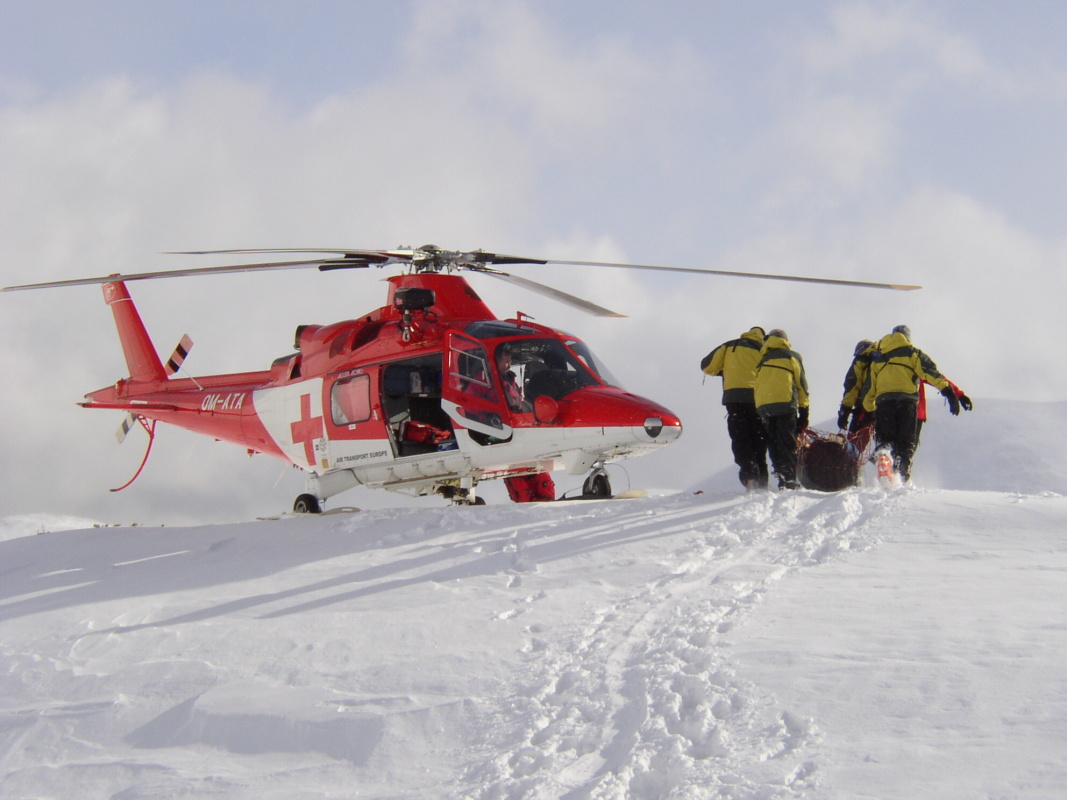
\includegraphics[height=6cm]{../figures/medical-evacuation}
        \end{center}
    \end{frame}

    \begin{frame}[fragile]
        \frametitle{Неформальная постановка задачи}
        \begin{center}
            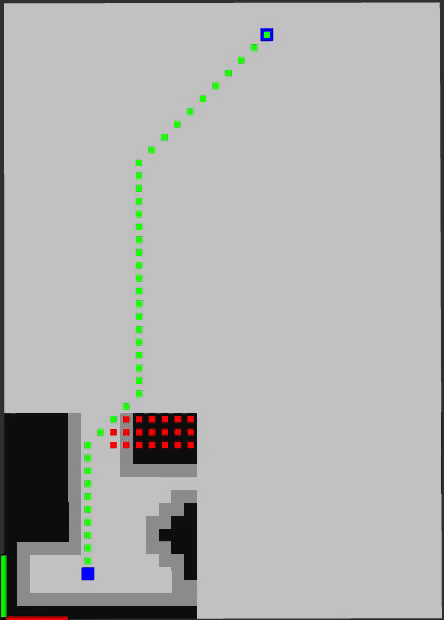
\includegraphics[height=5cm]{../figures/dstar8cells}
        \end{center}
    \end{frame}

    \begin{frame}[fragile]
        \frametitle{Постановка задачи -- обозначения}
        $G = (V, E)$ -- граф; $V$ --- конечное множество вершин, $E \subset V \times V \times \realpositive$ --- взвешенные ребра.

        $w: V \times V \rightarrow {\realpositive \lor \infty}$ -- функция веса ребра.

        $A = [v_1, v_2, \dots, v_n]: \forall i = 1, \dots, n-1$: $w(v_i, v_{i+1}) \neq \infty$  --- путь в графе.

        $P = P(V)$ --- множество путей в графе.

        $w(A) = \sum_{i = 1}^{n-1} w(v_i, v_{i+1})$ --- вес пути.

        $s(A)$ --- начало пути, $d(A)$ --- конец пути.

    \end{frame}

    \begin{frame}[fragile]
        \frametitle{Формальная математическая постановка задачи}

        Задача минимального пути --- нам даны вершины $s, d \in V$  (далее мы считаем, что $s, d, V$ фиксированы) и мы должны найти
        $$A_{plan}= \argmin_{\substack{A \subset V \text{ --- путь в } G \\ s(A) = s \\ d(A) = d}} w(A).$$
        Мы будем также говорить тогда, что $A = \mathtt{optpath}(G, s, d)$.

    \end{frame}

    \begin{frame}[fragile]
        \frametitle{Формальная алгоритмическая постановка задачи}

        Мы хотим решать задачу минимального пути \textit{онлайн} (longterm planning).
        Ее решение --- тройка $(T, \fplan, \fextract)$ из произвольного множества и двух вычислимых фукнций соответственно, такую что:
        \begin{align*}
            &\fempty \in T \\
            &\fplan: E \times T \rightarrow T \\
            &\fextract: T \rightarrow P(V) \\
            &\fextract(\fplan(E, \fempty)) = \mathtt{optpath}(G, s, d) \\
            &\fextract(t_0) = \mathtt{optpath}((V, E'), s, d) \rightarrow \\
            &\qquad \fextract(\fplan(E_{new}, t_0)) = \mathtt{optpath}((V, E' \leftarrow E_{new}), s, d)
        \end{align*}

    \end{frame}


    \begin{frame}
        \frametitle{Известные решения}
        \begin{itemize}
            \item Повторный A* на новых весах
            \item Dynamic SWSF-FP
            \begin{itemize}
                \item Переиспользует предыдущие результаты поиска
                \item $\approx$ BFS
            \end{itemize}
        \end{itemize}
    \end{frame}

    \begin{frame}
        \frametitle{Пересчет}
        \begin{figure}
            \centering
            \begin{subfigure}[b]{0.49\textwidth}
                \centering
                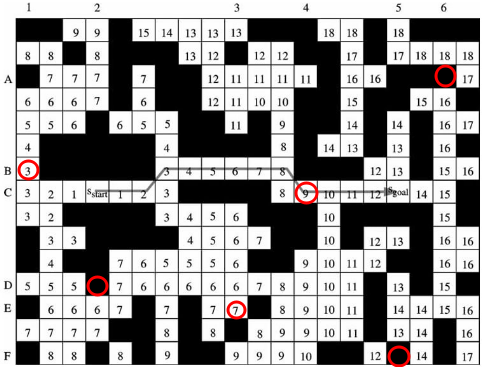
\includegraphics[width=\textwidth]{../figures/before-block.png}
            \end{subfigure}
            \hfill
            \begin{subfigure}[b]{0.49\textwidth}
                \centering
                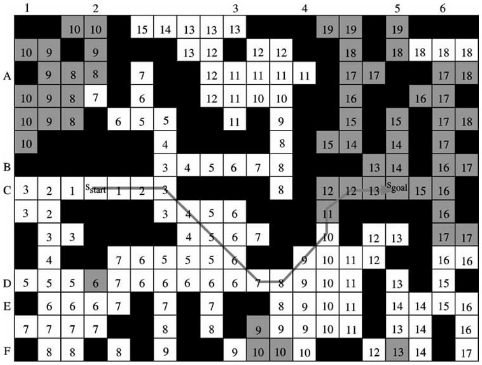
\includegraphics[width=\textwidth]{../figures/after-block.png}
            \end{subfigure}
        \end{figure}

    \end{frame}

    \begin{frame}
        \frametitle{Алгоритм LPA* --- идея}

        \begin{align*}
            &g^*(v) = \begin{cases}
                          0 &  v = s\\
                          \displaystyle \min_{v' \in neighbors(v)} (w(v, v') + g^*(v')) \\
            \end{cases} \\
            &rhs(v) = \min_{v' \in neighbors(v)} (w(v, v') + g(v')) \\ \\
            &rhs(v) = g(v)\ \forall v \in V \leftrightarrow g(v) = g^*(v)
        \end{align*}
        \begin{itemize}
            \item $rhs(v) \neq g(v)$ --- локальная неконсистентность
        \end{itemize}



    \end{frame}
    \begin{frame}[fragile]
        \frametitle{Алгоритм D* lite}
        \begin{verbatim}
g = init_graph()
while !agent.at_goal():
updates = receive_updated_edges_w()
replan_path(goal
    agent.pos
    g
    updates
    h) # LPA*
agent.step()
        \end{verbatim}

    \end{frame}

    \begin{frame}
        \frametitle{План экспериментов}
        \begin{itemize}
            \item Сравнить:
            \begin{itemize}
                \item Повторную A*
                \item DynamicSWSF-FP
                \item D* llite
            \end{itemize}
            \item На:
            \begin{itemize}
                \item Лабиринте
                \item Помещении
                \item Улице
            \end{itemize}
            \item Детали:
            \begin{itemize}
                \item Кардинальные ходы
                \item Датасет MovingAI
            \end{itemize}
        \end{itemize}
    \end{frame}

    \begin{frame}
        \frametitle{Ожидаемые результаты}
        Время работы (у.е.):
        \begin{table}[]
            \begin{tabular}{lllll}
                & Лабиринт & Помещение & Улица & \\
                A**             & $100x$   & $20y$     & $20z$ & \\
                Dynamic SWSF-FP & $2x$     & $2y$      & $2z$  & \\
                D* lite         & $x$      & $y$       & $z$   &
            \end{tabular}
        \end{table}

        Память (у.е.):
        \begin{table}[]
            \begin{tabular}{lllll}
                & Лабиринт & Помещение & Улица & \\
                A**             & $2x$     & $2y$      & $2z$  & \\
                Dynamic SWSF-FP & $x$      & $y$       & $z$   & \\
                D* lite         & $2x$     & $2y$      & $2z$  &
            \end{tabular}
        \end{table}


    \end{frame}

    \begin{frame}
        \frametitle{План работ}
        \begin{itemize}
            \item До 2 декабря --- написать кодовую основу для всего; преимущественно Максим
            \item До 16 декабря --- провести эксперименты и подготовить отчёт; преимущественно Лев
        \end{itemize}
    \end{frame}
\end{document}


